\section{Размерное квантование}
Квантоворазмерный эффект (квантовый размерный эффект) — изменение термодинамических и кинетических свойств кристалла, когда хотя бы один из его геометрических размеров становится соизмеримым с длиной волны де Бройля электронов. Этот эффект связан с квантованием энергии носителей заряда, движение которых ограничено в одном, двух или трёх направлениях.\\

Волны де Бройля — волны вероятности, определяющие плотность вероятности обнаружения объекта в заданной точке конфигурационного пространства. В соответствии с принятой терминологией говорят, что волны де Бройля связаны с любыми частицами и отражают их волновую природу.

\begin{gather} 
	\lambda = \frac{h}{p} = \frac{h}{\hbar k} = \frac{h}{mv};\\
	\psi(x, t) = A*e^{\frac{i}{\hbar}(px-Et)} = A*e^{i(kx-\omega t)}.
\end{gather}

В зависимости от размерности пространства электронный газ имеет различный закон дисперсии, плотность состояний и эффективную плотность состояний, см табл.~\ref{tab:gE}.

\begin{center}
    \begin{longtable}{| c | c | c | c |}
	    \caption{Плотность состояний и эффективная плотность состояний для низкоразмерных систем}
	    \label{tab:gE}
	    \\ \hline
	    Размерность & Закон дисперсии & $g(E)$ & $G(E)$ \\
	    \hline \endfirsthead
	    \subcaption{Продолжение таблицы~\ref{tab:gE}}
	    \\ \hline \endhead
	    \hline \subcaption{Продолжение на след. стр.}
	    \endfoot
	    \hline \endlastfoot
	    3D, bulk & $\frac{\hbar^{2}}{2m}(k_{x}^{2}+k_{y}^{2}+k_{z}^{2})$ & $ \frac{2^{\frac{1}{2}}m^{\frac{3}{2}}}{\pi^{2}\hbar^{3}}E^{\frac{1}{2}} $ & $\frac{(2m)^{\frac{3}{2}}}{3\pi^{2}\hbar^{3}}E^{\frac{3}{2}}$\\
	    \hline
	    2D, well & $\frac{\hbar^{2}}{2m}(k_{x}^{2}+k_{y}^{2})+\frac{\pi^{2}\hbar^{2}n^{2}}{2mL^{2}}$ & $\frac{m}{\pi\hbar^{2}}$ & $\frac{m}{\pi\hbar^{2}}E$\\
	    \hline
	    1D, wire & $\frac{\hbar^{2}}{2m}(k_{x}^{2}) + \frac{\pi^{2}\hbar^{2}}{2m}\Big( \frac{n_{1}^{2}}{L_{1}^{2}} + \frac{n_{2}^{2}}{L_{2}^{2}} \Big)$ & $\frac{\sqrt{m}}{\sqrt{2}\pi\hbar}E^{-\frac{1}{2}}$ & $\frac{\sqrt{2m}}{\pi\hbar}E^{\frac{1}{2}}$\\
	    \hline
	    0D, dot & $\frac{\pi^{2}\hbar^{2}}{2m}\Big( \frac{n_{1}^{2}}{L_{1}^{2}} + \frac{n_{2}^{2}}{L_{2}^{2}} + \frac{n_{3}^{2}}{L_{3}^{2}} \Big)$ & $2\delta E$ & $2$
    \end{longtable}
\end{center}

\begin{figure}[h]
	\centering
	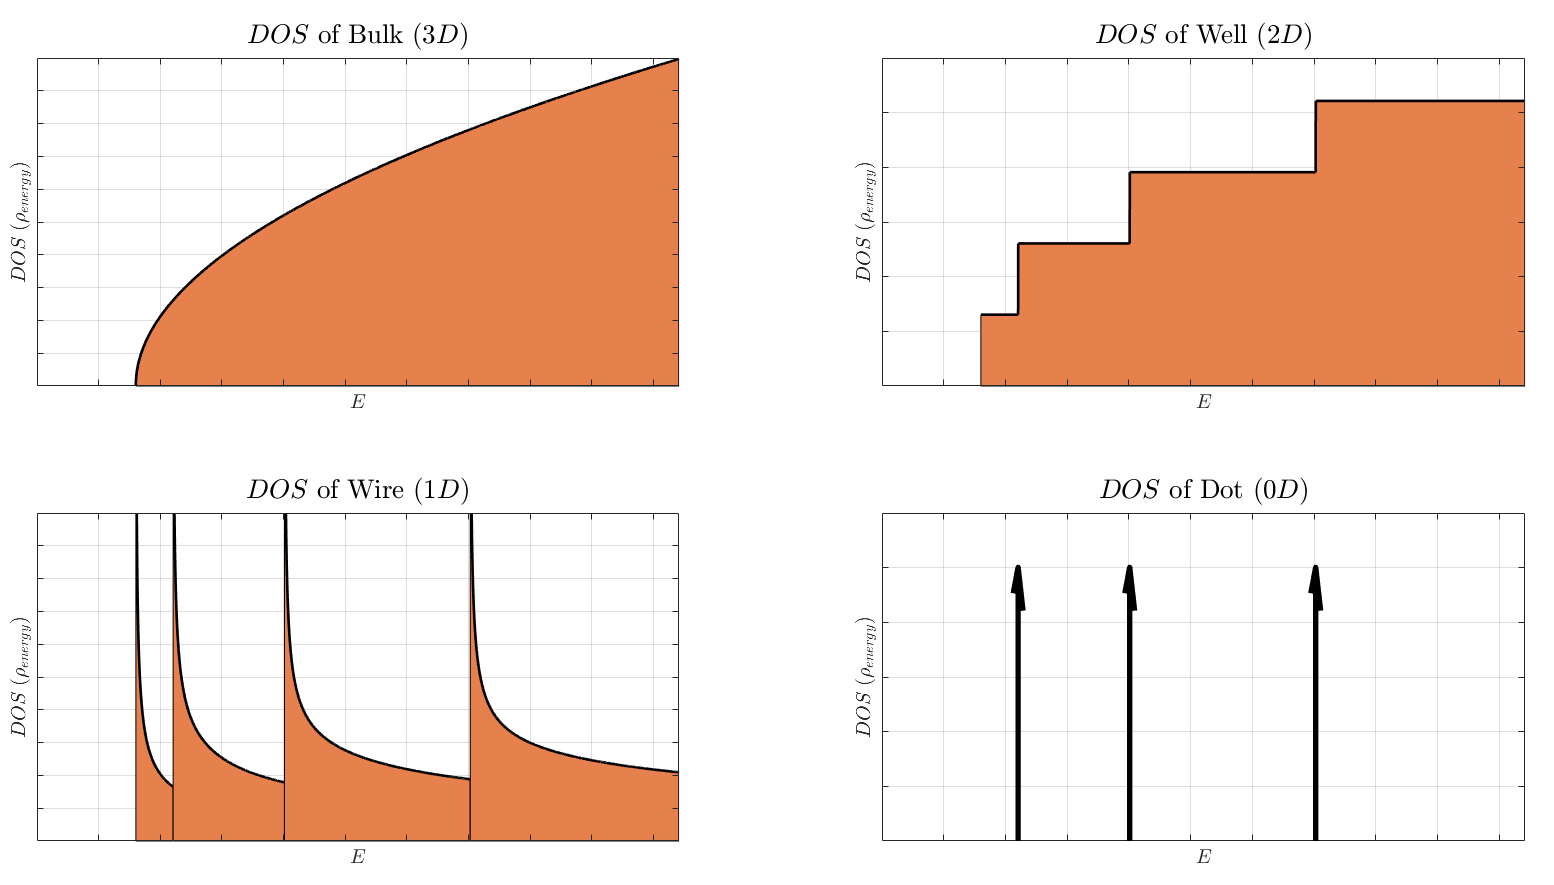
\includegraphics[width=\textwidth]{gE.png}
	\caption{Плотность состояний в 3D, 2D, 1D, 0D, где $g(E) = \rho_{energy}$}
	\label{DOS}
\end{figure}

\subsection{Трехмерное тело}
Рассмотрим 3D кристалл (bulk) на рис.~\ref{fig:3Dk}:
\begin{figure}[h]
	\centering
	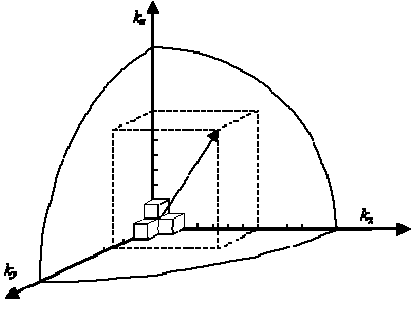
\includegraphics[scale=0.5]{3Dk.png}
	\caption{k-пространство (шар)}
	\label{fig:3Dk}
\end{figure}

Число состояний частицы $G(E)$ и плотность состояний $g(E)$, энергия которых не превышает некоторого фиксированного значения $E$, находятся из формул:
\begin{gather*} 
	G(E) = \frac{V_{sphere}}{V_{single-state}} = J_{z}\frac{\frac{1}{8}\frac{4}{3}\pi k^{3}}{\frac{\pi^3}{V}} = \frac{k^{3}V}{3\pi^{2}} = \frac{(2m)^{\frac{3}{2}}V}{3\pi^{2}\hbar^{3}}E^{\frac{3}{2}};\\
	k = \frac{\sqrt{2mE}}{\hbar};\\
	g(E) = \frac{dG(E)}{dE} = \frac{(2E)^{\frac{1}{2}}m^{\frac{3}{2}}}{\pi^{2}\hbar^{3}}V.
\end{gather*}

\subsection{Двухмерное тело}
Рассмотрим 2D кристалл (well) на рис.~\ref{fig:2Dk}:
\begin{figure}[h]
	\centering
	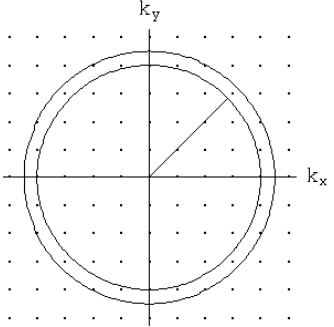
\includegraphics[scale=0.5]{2Dk.png}
	\caption{k-пространство (круг)}
	\label{fig:2Dk}
\end{figure}

\begin{gather*} 
	G(E) = \frac{V_{circul}}{V_{single-state}} = J_{z}\frac{\frac{1}{4}\pi k^{2}}{\frac{\pi^2}{S}} = \frac{k^{2}}{2\pi} = \frac{mS}{\pi\hbar^{2}}E;\\
	g(E) = \frac{dG(E)}{dE} = \frac{m}{\pi\hbar^{2}}S.
\end{gather*}

\subsection{Одномерное тело}
Рассмотрим 1D кристалл (wire)  на рис.~\ref{fig:1Dk}:
\begin{figure}[h]
	\centering
	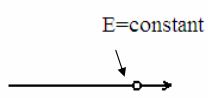
\includegraphics[scale=0.5]{1Dk.png}
	\caption{k-пространство (линия)}
	\label{fig:1Dk}
\end{figure}
\begin{gather*} 
	G(E) = \frac{V_{line}}{V_{single-state}} = J_{z}\frac{k}{\frac{\pi}{L}} = \frac{kL}{pi} = \frac{\sqrt{2m}L}{\pi\hbar}E^{\frac{1}{2}};\\
	g(E) = \frac{dG(E)}{dE} = \frac{\sqrt{m}L}{\sqrt{2}\pi\hbar}E^{-\frac{1}{2}}.
\end{gather*}

$J_{z}$ -- определяет число состояний не связанных с перемещением частицы в пространстве (например, число возможных проекций спина). В нашем случае, для электрона $J_{z}=2$.

% \section{Деградация}
% Деградация~--- процесс ухудшения характеристик какого-либо объекта c течением времени.

% Изучая деградацию гетероструктур (ГС) рассматривают следующие параметры:
% \begin{itemize}
% 	\item Вольт-амперная характеристика (ВАХ);
% 	\item Высота потенциального барьера (ПБ);
% 	\item Ширина потенциального барьера;
% 	\item Ширина потенциальной ямы (ПЯ);
% 	\item Т.д...
% \end{itemize}

% ГС используют для построения резонансно-туннельный диод (РТД), квантовых точек (КТ), транзисторов с высокой подвижностью электронов (HEMT) и так далее. 

% Химический состав ГС определяет ее зонную структуру, из чего вытекают особенности работы тех или иных устройств на ГС.

% Одна из причин деградации ВАХ ГС~--- диффузионное размытие профиля дна зоны проводимости ($E_{c}$). Некоторые факторы, от которых зависит диффузионное размытие:
% \begin{itemize}
% 	\item Химический состав; 
% 	\item Температура; 
% 	\item Время. 
% \end{itemize}

% Диффузионное размытие описывается с помощью законов Фика.

% % \section{Полупроводники}
% % Полупроводники (п/п)- широкий класс веществ, в которых концентрация подвижных носителей заряда значительно ниже, чем концентрация атомов, и может изменяться под влиянием температуры. освещения или относительно малого количества примесей.

% % Эффективная плотность состояний в зоне проводимости (ЗП)~\cite{MFTIne}:
% % \begin{equation}
% % 	N_{c} = 2\Big[ \frac{2\pi m_{e}^{\ast}k_{B}T}{h^{2}} \Big]
% % 	^{\frac{3}{2}},
% % \end{equation}
% % \begin{conditions}
% % 	$m_{e}^{\ast}$ & эффективная масса электрона;\\
% % 	$k_{B}$ & константа Больцмана;\\
% % 	$h$ & постоянная Планка;\\
% % 	$T$ & температура.
% % \end{conditions}

% % Эффективная плотность состояний в валентной зоне (ВЗ)~\cite{MFTIne}:
% % \begin{equation}
% % 	N_{v} = 2\Big[ \frac{2\pi m_{h}^{\ast}k_{B}T}{h^{2}} \Big]
% % 	^{\frac{3}{2}},
% % \end{equation}
% % \begin{conditions}
% % 	$m_{h}^{\ast}$ & эффективная масса дырки.
% % \end{conditions}

% % \subsection{Собственные полупроводники}
% % Собственный полупроводник (п/п i-типа)~--- это чистый полупроводник, содержание посторонних примесей в котором не превышает $10^{−8} … 10^{−9}\%$.

% % Концентрация собственных носителей заряда в ЗП~\cite{MFTIne}:
% % \begin{equation}
% % 	n_{i} = \sqrt{N_{c}N_{v}}\exp\!\bigg[ - \frac{E_{g}}{2k_{B}T} \bigg],
% % \end{equation}
% % \begin{conditions}
% % 	$E_{g}$ & ширина запрещенной зоны (ЗЗ) п/п.
% % \end{conditions}

% % \subsection{Примесные полупроводники}
% % Примесный полупроводник - это полупроводник электрофизические свойства которого определяются, в основном, примесями других химических элементов.

% % Концентрация электронов в ЗП примесного п/п ~\cite{MFTIne}:
% % \begin{equation}
% % 	n = \frac{N_{D}}{2}\bigg( 2 + \frac{1}{2}\bigg( \frac{2n_{i}}{N_{D}} \bigg)^{2} \bigg),
% % \end{equation}
% % \begin{conditions}
% % 	$N_{D}$ & концентрация атомов легирующей примеси.
% % \end{conditions}

% \subsection{Зонная диаграмма гетероперехода}
% Для построения зонной диаграммы необходимо знать ширину запрещенной зоны ($E_{g}$) и положение уровня Ферми ($E_{F}$) для контактируемых полупроводников.

% \begin{figure}[h]
%   \centering
%   \includegraphics[width=.5\linewidth]{assets/Eg}
%   \caption{Зонная диаграмма перехода между полупроводниками с различными $E_{g}$}
%   \label{img:2.0.0}
% \end{figure}

% Одна из самых распространенных ГС~--- это ГС на основе твердого раствора $Al_{x}Ga_{1−x}As$, где $x$ -- это доля замещения.
% Основные характеристики $Al_{x}Ga_{1−x}As$:

% \begin{center}
%   \begin{longtable}{|c|c|}
%     \caption{Основные параметры $Al_{x}Ga_{1−x}As$}
%     \label{tab:2.0.0}
%     \\ \hline
%     Параметр & $Al_{x}Ga_{1−x}As$ \\
%     \hline \endfirsthead
%     \subcaption{Продолжение таблицы~\ref{tab:2.0.0}}
%     \\ \hline \endhead
%     \hline \subcaption{Продолжение на след. стр.}
%     \endfoot
%     \hline \endlastfoot
% 	Кристаллическая структура& Типа цинковой обманки \\ \hline
% 	Постоянная решетки $a[nm]$  & $0.56533+0.00078x$ \\ \hline
% 	$E_{g}^{\Gamma}[eV],\, x < 0.45$    & $1.424+1.247x$ \\ \hline
% 	$E_{g}^{\Gamma}[eV],\, x > 0.45$    & $1.656+0.215x+0.143x^{2}$ \\ \hline
% 	% $\Delta E_{c}^{\Gamma}[eV],\, x < 0.45$    & $0.773x$ \\ \hline
% 	% $\Delta E_{c}^{\Gamma}[eV],\, x > 0.45$    & $0.232-0.259x+1.147x^{2}$ \\ \hline
% 	$m_{e}^{\Gamma}$    & $0.067+0.083x$ \\ \hline
% 	$m_{lh}$    & $0.082+0.071x$ \\ \hline
% 	$N_{atoms}[1/sm^{-3}]$    & $(4.42-0.17x)10^{22}$
%   \end{longtable}
% \end{center}

% Следует также принимать во внимание, что полупроводники могут иметь минимумы зоны проводимости в разных точках зоны Брюллиена. К примеру, минимум зоны проводимости $GaAs$ находится в точке $\Gamma$, в то время как наименьший минимум в $AlAs$ близок к точке $X$. Таким образом, природа низшего минимума зоны проводимости меняется при изменении доли $Al$ в твердом растворе $Al_{x}Ga_{1−x}As$. Низший минимум в $Al_{x}Ga_{1−x}As$ изменяется от прямого расположения (минимум в $\Gamma$) зон до непрямой зонной структуры (минимум в $Х$) при содержании $Al \approx 45\%$. Обычно твердый раствор $Al_{x}Ga_{1−x}As$ получают с долей $Al$, меньше $0.45$, чтобы получить прямое расположение зон.

% Рассматривая ГП $i\!-\!GaAs/i\!-\!Al_{x}Ga_{1−x}As$, при $x < 0.45$, получим высоту потенциальной ступеньки в зоне проводимости ($E_{c2} - E_{c1}$) $U \approx 1.247*x\, eV$.
% \section{Конкретная структура на основе $Al_{x}Ga_{1−x}As$}

% Более подробно рассмотрим гетероструктуру на основе $Al_{x}Ga_{1−x}As$. Возьмем $GaAl$/$AlAs$/$GaAl$/$AlAs$/$GaAl$, с соответствующими размерами $8$/$4$/$6$/$4$/$8$ -- монослоев.